\documentclass{article}

\usepackage{graphicx}

\title{Report 2}
\author{Aanjishnu Bhattacharyya}

\begin{document}
\maketitle

\section{Attempt to Denoise}

The audio data that is recorded is filled with external noise, like engine growl, people speaking and such. To combat this a simple de-noising scheme was implemented, pre-emphasizing the noise followed by FFT unwanted frequency reduction. This reduces the noise to signal ratio. But overall prediction suffers because \textbf{YAMNet} is trained on extrmely noisy data. Will try with other types of pre-trained network.

\begin {figure}[h]
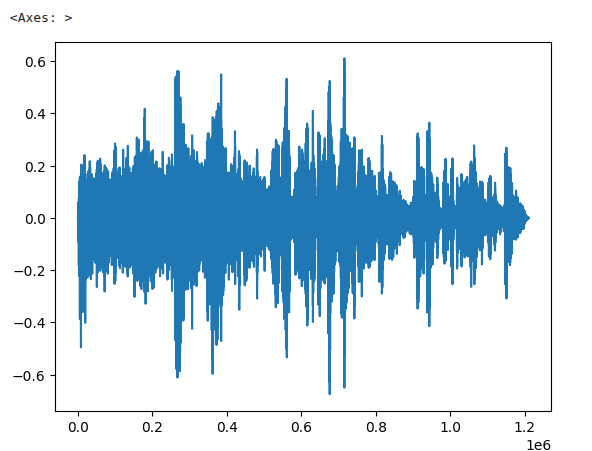
\includegraphics[width=\textwidth]{foo1.png}
\caption{Original}
\end {figure}
\begin {figure}[h]
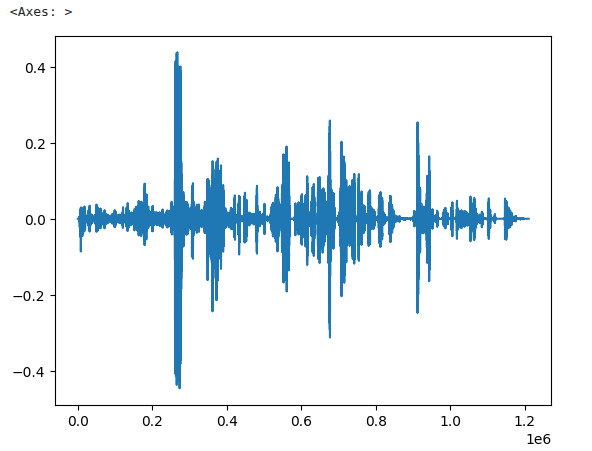
\includegraphics[width=\textwidth]{foo2.png}
\caption{Denoised}
\end {figure}

\section{Filtering and PCA with $n\_components>2$}

To improve the prediction capibilities of the system, I impletemend filtering as discussed, removing the \textit{Transformer} from the loop to avoid haluciantion. A Mode based measure was utilized to predict if the value is actually a horn.

\begin {figure}[h]
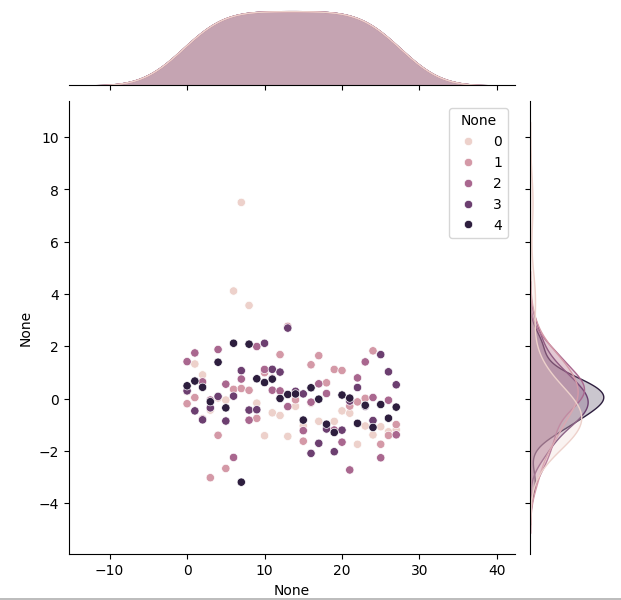
\includegraphics[width=\textwidth]{foo3.png}
\caption{PCA with $n\_components=5$}
\end {figure}

To improve the chances of prediction we include other unrelated values aswell, \textit{Siren}, \textit{Alarm}, \textit{Buzzer}. To increase the broad classification range. 

Principle component analysis works extrmely well for n\_components with a value of 5.


\section{K-Means and HDBSCAN}

K-Means Clustering performed better than the original Birch alorithm. HDBSCAN was also able to identify values which are not classifiable. Marked out with the value of -1.

The graphs are based on PCA-2 so that we can display the graphs.

\begin {figure}[h]
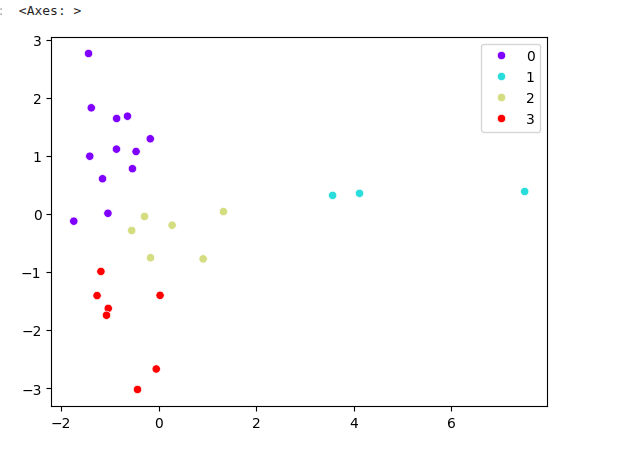
\includegraphics[width=\textwidth]{kmeanns.png}
\caption{K-means based on PCA-2}
\end {figure}

\begin {figure}[h]
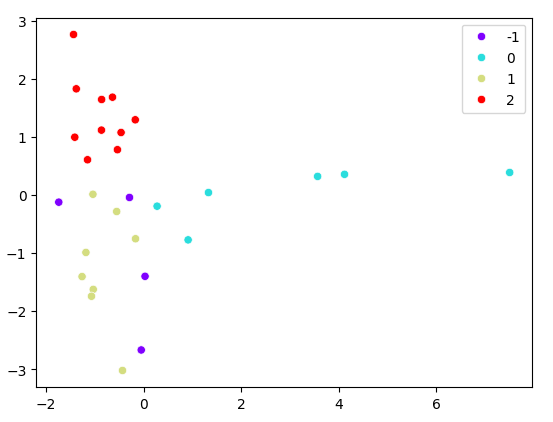
\includegraphics[width=\textwidth]{hdbscan.png}
\caption{HDBSCAN based on PCA-2}
\end {figure}

\section{Labeling of data}
A bunch of data point have been labeled, I downloaded data from \textit{freesound.org}, \textit{BBC Sound} and Other manufacturer sites. I will label further.

\end{document}
